% This is "sig-alternate.tex" V2.1 April 2013
% This file should be compiled with V2.5 of "sig-alternate.cls" May 2012
%
% This example file demonstrates the use of the 'sig-alternate.cls'
% V2.5 LaTeX2e document class file. It is for those submitting
% articles to ACM Conference Proceedings WHO DO NOT WISH TO
% STRICTLY ADHERE TO THE SIGS (PUBS-BOARD-ENDORSED) STYLE.
% The 'sig-alternate.cls' file will produce a similar-looking,
% albeit, 'tighter' paper resulting in, invariably, fewer pages.
%
% ----------------------------------------------------------------------------------------------------------------
% This .tex file (and associated .cls V2.5) produces:
%       1) The Permission Statement
%       2) The Conference (location) Info information
%       3) The Copyright Line with ACM data
%       4) NO page numbers
%
% as against the acm_proc_article-sp.cls file which
% DOES NOT produce 1) thru' 3) above.
%
% Using 'sig-alternate.cls' you have control, however, from within
% the source .tex file, over both the CopyrightYear
% (defaulted to 200X) and the ACM Copyright Data
% (defaulted to X-XXXXX-XX-X/XX/XX).
% e.g.
% \CopyrightYear{2007} will cause 2007 to appear in the copyright line.
% \crdata{0-12345-67-8/90/12} will cause 0-12345-67-8/90/12 to appear in the copyright line.
%
% ---------------------------------------------------------------------------------------------------------------
% This .tex source is an example which *does* use
% the .bib file (from which the .bbl file % is produced).
% REMEMBER HOWEVER: After having produced the .bbl file,
% and prior to final submission, you *NEED* to 'insert'
% your .bbl file into your source .tex file so as to provide
% ONE 'self-contained' source file.
%
% ================= IF YOU HAVE QUESTIONS =======================
% Questions regarding the SIGS styles, SIGS policies and
% procedures, Conferences etc. should be sent to
% Adrienne Griscti (griscti@acm.org)
%
% Technical questions _only_ to
% Gerald Murray (murray@hq.acm.org)
% ===============================================================
%
% For tracking purposes - this is V2.0 - May 2012

\documentclass{sig-alternate-05-2015}
\graphicspath{{./figure/}}
\usepackage{Definitions}
\usepackage[colorlinks=true]{hyperref}


\begin{document}

% Copyright
\setcopyright{acmcopyright}
%\setcopyright{acmlicensed}
%\setcopyright{rightsretained}
%\setcopyright{usgov}
%\setcopyright{usgovmixed}
%\setcopyright{cagov}
%\setcopyright{cagovmixed}


% DOI
\doi{10.475/123_4}

% ISBN
\isbn{123-4567-24-567/08/06}

%Conference
\conferenceinfo{PLDI '13}{June 16--19, 2013, Seattle, WA, USA}

\acmPrice{\$15.00}

%
% --- Author Metadata here ---
\conferenceinfo{WOODSTOCK}{'97 El Paso, Texas USA}
%\CopyrightYear{2007} % Allows default copyright year (20XX) to be over-ridden - IF NEED BE.
%\crdata{0-12345-67-8/90/01}  % Allows default copyright data (0-89791-88-6/97/05) to be over-ridden - IF NEED BE.
% --- End of Author Metadata ---

\title{Neural Marked Temporal Point Process \\ with Applications to Human Activities Predictions}

%
% You need the command \numberofauthors to handle the 'placement
% and alignment' of the authors beneath the title.
%
% For aesthetic reasons, we recommend 'three authors at a time'
% i.e. three 'name/affiliation blocks' be placed beneath the title.
%
% NOTE: You are NOT restricted in how many 'rows' of
% "name/affiliations" may appear. We just ask that you restrict
% the number of 'columns' to three.
%
% Because of the available 'opening page real-estate'
% we ask you to refrain from putting more than six authors
% (two rows with three columns) beneath the article title.
% More than six makes the first-page appear very cluttered indeed.
%
% Use the \alignauthor commands to handle the names
% and affiliations for an 'aesthetic maximum' of six authors.
% Add names, affiliations, addresses for
% the seventh etc. author(s) as the argument for the
% \additionalauthors command.
% These 'additional authors' will be output/set for you
% without further effort on your part as the last section in
% the body of your article BEFORE References or any Appendices.

\numberofauthors{8} %  in this sample file, there are a *total*
% of EIGHT authors. SIX appear on the 'first-page' (for formatting
% reasons) and the remaining two appear in the \additionalauthors section.
%
%\author{
%% You can go ahead and credit any number of authors here,
%% e.g. one 'row of three' or two rows (consisting of one row of three
%% and a second row of one, two or three).
%%
%% The command \alignauthor (no curly braces needed) should
%% precede each author name, affiliation/snail-mail address and
%% e-mail address. Additionally, tag each line of
%% affiliation/address with \affaddr, and tag the
%% e-mail address with \email.
%%
%% 1st. author
%\alignauthor
%Ben Trovato\titlenote{Dr.~Trovato insisted his name be first.}\\
%       \affaddr{Institute for Clarity in Documentation}\\
%       \affaddr{1932 Wallamaloo Lane}\\
%       \affaddr{Wallamaloo, New Zealand}\\
%       \email{trovato@corporation.com}
%% 2nd. author
%\alignauthor
%G.K.M. Tobin\titlenote{The secretary disavows
%any knowledge of this author's actions.}\\
%       \affaddr{Institute for Clarity in Documentation}\\
%       \affaddr{P.O. Box 1212}\\
%       \affaddr{Dublin, Ohio 43017-6221}\\
%       \email{webmaster@marysville-ohio.com}
%% 3rd. author
%\alignauthor Lars Th{\o}rv{\"a}ld\titlenote{This author is the
%one who did all the really hard work.}\\
%       \affaddr{The Th{\o}rv{\"a}ld Group}\\
%       \affaddr{1 Th{\o}rv{\"a}ld Circle}\\
%       \affaddr{Hekla, Iceland}\\
%       \email{larst@affiliation.org}
%\and  % use '\and' if you need 'another row' of author names
%% 4th. author
%\alignauthor Lawrence P. Leipuner\\
%       \affaddr{Brookhaven Laboratories}\\
%       \affaddr{Brookhaven National Lab}\\
%       \affaddr{P.O. Box 5000}\\
%       \email{lleipuner@researchlabs.org}
%% 5th. author
%\alignauthor Sean Fogarty\\
%       \affaddr{NASA Ames Research Center}\\
%       \affaddr{Moffett Field}\\
%       \affaddr{California 94035}\\
%       \email{fogartys@amesres.org}
%% 6th. author
%\alignauthor Charles Palmer\\
%       \affaddr{Palmer Research Laboratories}\\
%       \affaddr{8600 Datapoint Drive}\\
%       \affaddr{San Antonio, Texas 78229}\\
%       \email{cpalmer@prl.com}
%}
% There's nothing stopping you putting the seventh, eighth, etc.
% author on the opening page (as the 'third row') but we ask,
% for aesthetic reasons that you place these 'additional authors'
% in the \additional authors block, viz.
%\additionalauthors{Additional authors: John Smith (The Th{\o}rv{\"a}ld Group,
%email: {\texttt{jsmith@affiliation.org}}) and Julius P.~Kumquat
%(The Kumquat Consortium, email: {\texttt{jpkumquat@consortium.net}}).}
%\date{30 July 1999}
% Just remember to make sure that the TOTAL number of authors
% is the number that will appear on the first page PLUS the
% number that will appear in the \additionalauthors section.

\maketitle
\begin{abstract}
Human activities constantly produce temporal-spatial sequences of events ranging from social interactions to financial transactions to electronic medical records. Are these activities predictable ? Can we forecast which activity people might take at what time in the future based on his (her) past history ? In this paper, we propose a novel random process, referred to as the Neural Marked Temporal Point Process, to take into account both the discrete action prediction (classification) task and the continuous time prediction (regression) task in a unified framework. An innovative feature of the proposed model is that we apply a Recurrent Neural Network to learn a unified representation of the past activities and time, conditioned on which we can jointly formulate the probability of the next activity and the density of the respective temporal interval. This new model establishes a previously under-explored general connection between recurrent neural network and marked temporal point process. We have conducted large-scale experiments on both synthetic and real world time series data and demonstrate that Neural Marked Temporal Point Process can capture meaningful dependency over the historical data, which leads to consistently better prediction performance compared to alternative competitors. 
\end{abstract}


%
% The code below should be generated by the tool at
% http://dl.acm.org/ccs.cfm
% Please copy and paste the code instead of the example below. 
%
\begin{CCSXML}
<ccs2012>
 <concept>
  <concept_id>10010520.10010553.10010562</concept_id>
  <concept_desc>Computer systems organization~Embedded systems</concept_desc>
  <concept_significance>500</concept_significance>
 </concept>
 <concept>
  <concept_id>10010520.10010575.10010755</concept_id>
  <concept_desc>Computer systems organization~Redundancy</concept_desc>
  <concept_significance>300</concept_significance>
 </concept>
 <concept>
  <concept_id>10010520.10010553.10010554</concept_id>
  <concept_desc>Computer systems organization~Robotics</concept_desc>
  <concept_significance>100</concept_significance>
 </concept>
 <concept>
  <concept_id>10003033.10003083.10003095</concept_id>
  <concept_desc>Networks~Network reliability</concept_desc>
  <concept_significance>100</concept_significance>
 </concept>
</ccs2012>  
\end{CCSXML}

\ccsdesc[500]{Computer systems organization~Embedded systems}
\ccsdesc[300]{Computer systems organization~Redundancy}
\ccsdesc{Computer systems organization~Robotics}
\ccsdesc[100]{Networks~Network reliability}


%
% End generated code
%

%
%  Use this command to print the description
%
\printccsdesc

% We no longer use \terms command
%\terms{Theory}

\keywords{Recurrent neural network; Marked point process; Time series; Stochastic process}

\section{Introduction}
Temporal-spatial event data have been becoming ubiquitous due to the fast development of modern communications, mobile devices, and various wearable gadgets. 
%
Large collections of these data arise from social activities, to financial transactions, to electronic health records, which provide rich information about what type of event is happening between which entities at what time and place. 
%
Quite often, each set of temporal events associated with an involved entity (online user, stock ID, patients) is first ordered by time and then chained together to form a temporal sequence. The resulting collection of sequences capture the full traces of historical activities induced from the respective entities over time.
%
For instance, people go to work, airports, gas stations, parks, cinemas, church, restaurants, groceries at different time of days in a week. Music streaming subscribers listen to different albums and watch various videos as time goes by. Professional trading systems buy and sell a bunch of stocks within short-time frames. Patients go to see the doctor with a time-stamped sequence of diagnoses of the concerned diseases. 

\begin{figure}
	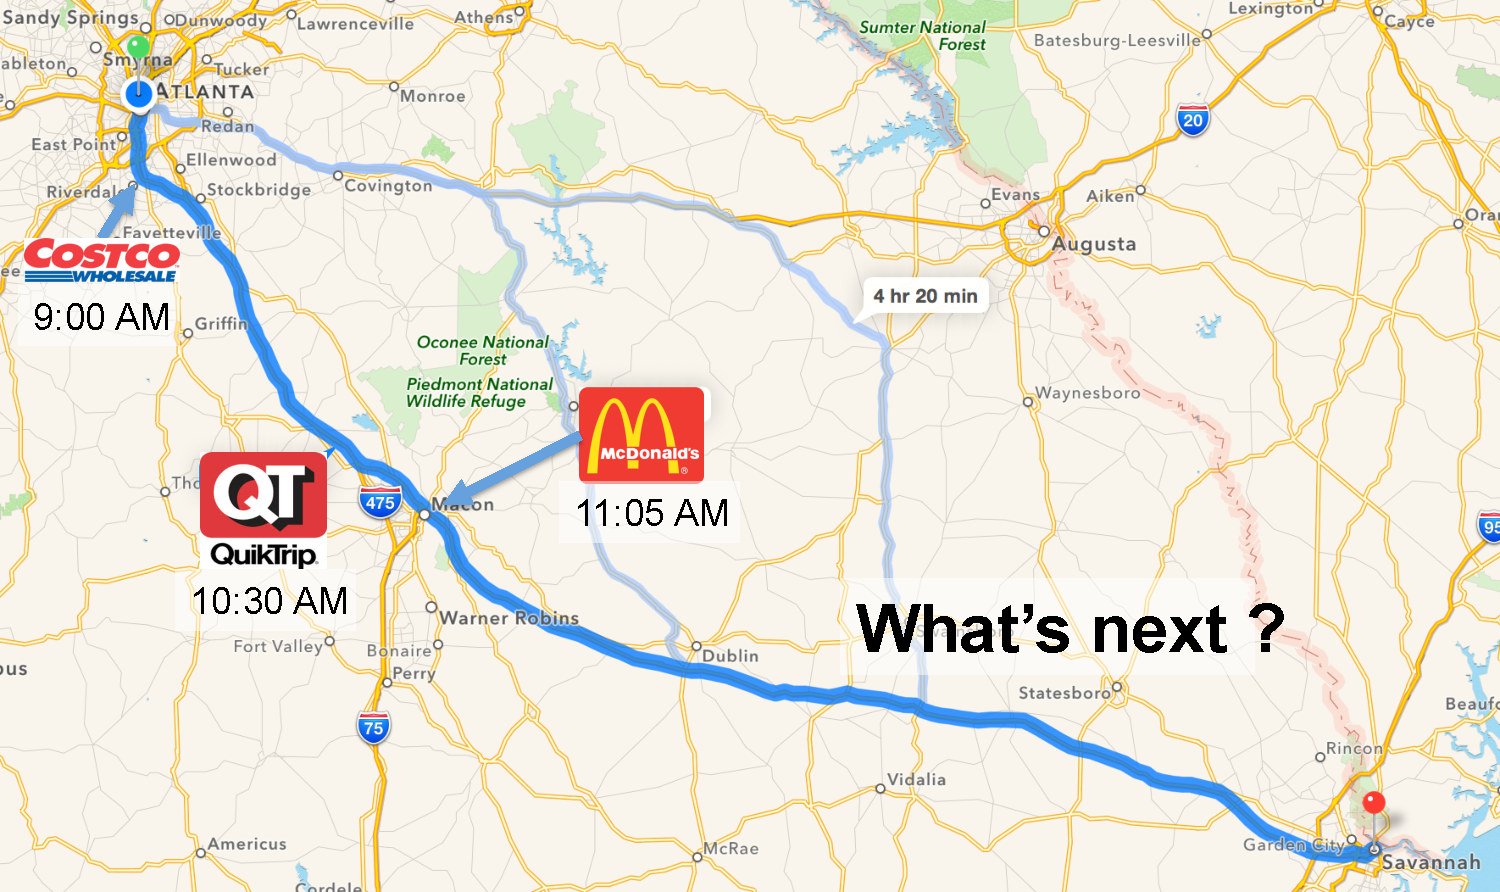
\includegraphics[width=\columnwidth]{fig1}
	\caption{A user has visited Costco at 9:00AM, refilled the gas in QT at 10:30AM, and then had lunch in MacDonald at 11:05AM. Given the trace of these past locations and time, can we predict what the next stop will be and when it will happen in the future ? \label{demo}} 
\end{figure}
Although the aforementioned situations come from different domains, we seek to capture them in a unified framework by addressing the key problem : can human activities be predictable ? Based on the sequence of past events, can we predict what kind of action people will take at what time in the future ? Accurately predicting the next activity at the right moment will have potential applications of great significance. For mainstream personal assistants, shown in Figure~\ref{demo}, because people tend to visit different places dependent on the temporal/spatial contexts like morning vs. evening, weekdays vs. weekend, successfully predicting the next places that users will visit at the most likely time will make such services more relevant and usable. In stock market, accurately forecasting when to sell or buy a particular stock next means critical business success. Finally, for modern healthcare, patients may have several diseases that have complicated dependencies on each other. The occurrence of one disease can trigger the progression of others. Accurately estimating when a probable disease might occur can effectively help to take proactive steps to reduce the potential risks in the future. 

Existing studies in literature attempt to solve this problem from two different perspectives. On the one hand, classic varying-order Markov models formulate the problem as a discrete-time sequence prediction task. Based on the history, they seek to predict the most likely state the process will go into on the next step. As a result, one limit of the Markov model is that it assumes the process proceeds by a unit time-step, so it cannot capture the heterogeneity of the time to predict the timing of the next event in the future. Furthermore, when the number of states is large, Markov model cannot have long dependency on the history since the overall state-space will grow exponentially. Semi-Markov model can capture the continuous interval between two successive states to some extent by assuming the intervals have exponential distribution. But still, it has the same state-space explosion issue when the order grows. On the other hand, classic marked temporal point process explicitly treat the time interval between two activities as continuous random variable. The type of each event can be modeled either as an explicit marker or as an independent dimension. However, most studies along this line are restricted to low dimension and small data settings for simple inference problems. The high dimensional nature, the complexity of the event features, the sheer volume of the data, and particularly the unique learning problems faced by modern emerging applications such as the ones mentioned above pose new great challenges in their modeling and learning. Therefore, in this work, we propose a novel random process, referred to as the Neural Marked Temporal Point Process, to take into account both sources of information from event types and timing to make future predictions. More precisely, we make the following contributions :
\begin{itemize}
\item We establish a previously under explored connection between Recurrent Neural Networks and Marked Temporal Point Processes, which enables joint predictions of event type and timing in the future by incorporating the long-term influence of the past history.

\item We point out that the proposed Neural Marked Temporal Point Process has implications beyond temporal-spatial features and sequence predictions. We will show that our construction can be generalized to other settings by incorporating more rich contextual information and features.

\item We conduct large-scale experiments on both synthetic and real-world datasets from a diverse range of domains to show that our model have consistently better predictive performance for both the event type and timing  compared to alternative competitors. 

\end{itemize}
 
\section{Related Work}
This will include several related studies from varying Markov models, Semi-Markov models, RNN, LSTM, GRU, Temporal Point Process, Marked Temporal Point Process

\section{Human Activities Predictions}
\subsection{Problem Definition}
Graphical Model Representation
\subsection{Marked Temporal Point Process}
\subsection{Recurrent Neural Network}
\subsection{Neural Marked Temporal Point Process}

\section{Experiments}
\subsection{Synthetic Data}
1. only considers time : autoregressive point process with exponential, Rayleigh duration distribution; Single Hawkes Process
2. Considers time and marker jointly : two dimensional Hawkes process, graphical models
\subsection{Real Data}
1. Stock, MIMIC2, NY Taxi, Alibaba, LastFM, StackOverFlow
2. Empirical patterns found in data : interval distributions (by week day vs. by weekend), history correlations (whether history will help), QQ-plot, 
3. Visualization of NY Taxi, Visualization of RNN predictions
\section{Discussions}
extend to consider other features, like spatial information, structure information
\section{Conclusions}

\end{document}
